\chapter{Rahmenentfernung}

\begin{figure}[h]
 	$
 	G = \frac{1}{159}
	\begin{bmatrix}
		2 & 4 & 5 & 4 & 2 \\ 
		4 & 9 & 12 & 9 & 4 \\
		5 & 12 & 15 & 12 & 5 \\
		4 & 9 & 12 & 9 & 4 \\
		2 & 4 & 5 & 4 & 2 \\
	\end{bmatrix},	
	$
	$
	C_x = 
	\begin{bmatrix}
	-1 & 0 & +1 \\
	-2 & 0 & +2 \\
	-1 & 0 & +1
	\end{bmatrix},
	$
	$	
	C_y = 
	\begin{bmatrix}
	-1 & -2 & -1 \\
	0 & 0 & 0 \\
	+1 & +2 & +1
	\end{bmatrix},
	$
\caption{Die Figur zeigt den Gausfilterkernel sowie die Faltungsmasken, die beim Canny-Algorithmus verwendet werden}
\label{fig:gauss}
\end{figure}

Die Extraktion eines Bildes aus einem monotonen Rahmen geschieht in mehreren Schritten. Zu Beginn wird das gesamte Bild mit dem Canny-Kantendetektionsalgorithmus in ein binär Bild umgewandelt, dass sämtliche Pixel weiß darstellt bei denen eine hoher unterschied in der Intensität festzustellen ist. Dazu wird in dem Bild rauschen durch einen Gaußfilter entfernt dessen Kernel in Abbildung \ref{fig:gauss} zu erkennen ist. Um dann die Gradienten des Bildes mit zwei Faltungsmasken zu bestimmen, die auch in Abbildung \ref{fig:gauss} dargestellt sind. Die so gewonnen Gradienten werden durch eine Non-Maximum surpression überprüft, ob sie teil einer Kante sind. Daraus resultieren nur dünne Linien (\cite{OpenCVCanny}). Bei anderen Kantendetektoren wird dieser Schritt nicht ausgeführt, was im späteren dazu führen kann, dass es schwerer wird den Rahmen des Bildes zu erkennen.
 
Das Ergebnis des Canny-Kantendetektionsalgorithmus hat dann die Eigenschaft, dass stellen des Bildes mit einer monotonen Fläche nur schwarz sind und dort keine starken Gradienten durch weiße Pixel markiert wurden. Mit Hilfe dieser Eigenschaft kann man einen monotonen Rahmen um das gegebene Bild erkennen. Hierzu betrachtet man jede Seite des Bildes einzeln und betrachtet für jede Seite einen bestimmten Ausschnitt. Das erste Fenster, das betrachtet wird, hat die Höhe beziehungsweise Breite der gewählten Seite des Bildes und geht eine gegebene Anzahl von Pixeln in das Bild. Nun kann man innerhalb dieses Fensters die weißen Pixel zählen. Nachdem dies geschehen ist vergrößert man den Ausschnitt indem man weitere reihen an Pixeln des Bildes hinzunimmt und man wieder die weißen Pixel zählt. Im Schaubild \ref{fig:bordergradient} sind die Ergebnisse eines solchen Vorgehens für ein Bild mit monotonem Rahmen dargestellt. Man kann deutlich erkennen, dass die Steigung deutlich abnimmt sobald der Rahmen erreicht ist. Direkt nach dem Rahmen nimmt die Steigung wieder zu. Der Rahmen muss sich dort befinden wo der Gradient am geringsten ist und endet an dem Punkt, wo der Gradient einen Ausschlag nach oben macht. Dies kann man an den gezeichneten Gradienten in dem Schaubild \ref{fig:bordergradient} erkennen. Um danach den Rahmen zu entfernen schneidet man das Bild an dieser Stelle aus.    

\begin{figure}
	\centering
	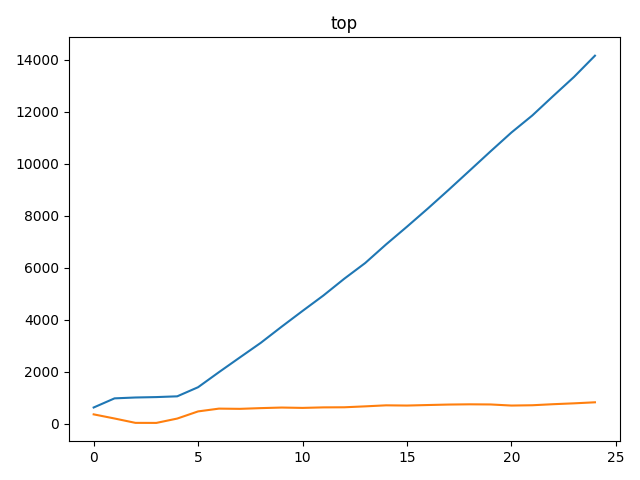
\includegraphics[width=0.3\linewidth]{images/plot_frame/plot_top_frame.png}
	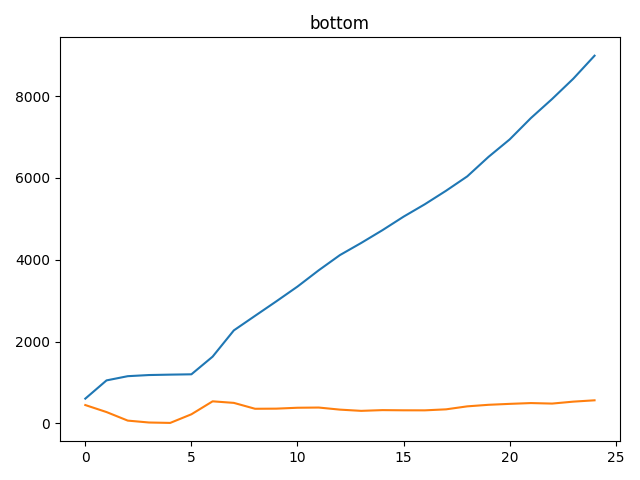
\includegraphics[width=0.3\linewidth]{images/plot_frame/plot_bottom_frame.png}\\
	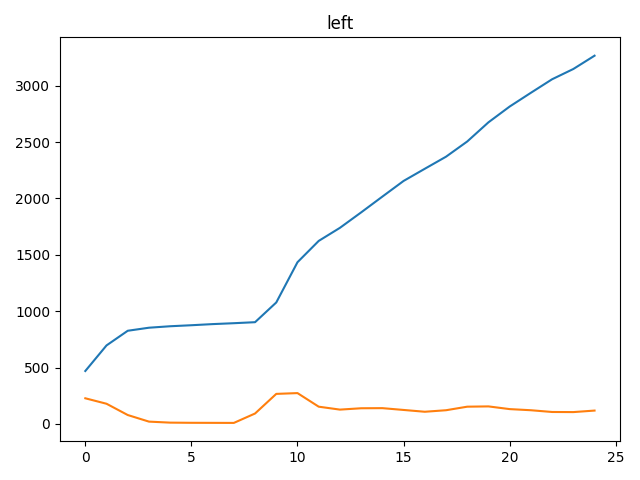
\includegraphics[width=0.3\linewidth]{images/plot_frame/plot_left_frame.png}
	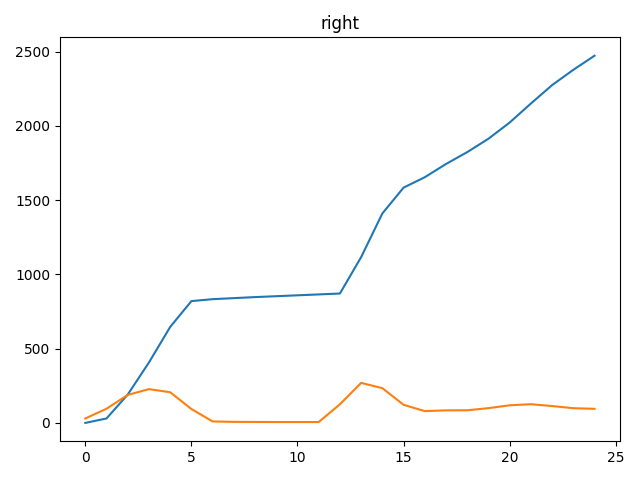
\includegraphics[width=0.3\linewidth]{images/plot_frame/plot_right_frame.png}
	\caption{Die Diagramme zeigen in der oberen Linie die Zunahme der weißen Pixel in den immer größer werdenden Fenstern. Außerdem zeigen sie die jeweiligen Gradienten zur vorhergehenden Anzahl an weißen Pixeln in der darunter liegenden Linie.}
	\label{fig:bordergradient}
\end{figure}    